\section{Case Studies}\label{sec:casestudy}

The algorithmic story is useful only if the \(r=1\) target is useful.
%
This section therefore asks a practical question:
when an analyst wants vertex-level cohesive structure, is \((1,s)\) enough?
%
On the ground-truth tasks reported here, \((1,s)\) matches the quality of higher-\(r\) nuclei on the evaluated metrics while costing much less.
%
The claim is empirical and scoped to these datasets and metrics.

\stitle{Setup.}\label{sec:cs-setup}
For cross-\(r\) comparisons, we use the standard \((r,s)\)-nucleus parameterization~\cite{nucleusSariyuce14}.
%
The paper's algorithmic results apply only to \(r=1\).
%
The \(r=2\) and \(r=3\) results are baselines from the same nucleus family.
%
Because those baselines score edges or triangles, we project their scores to vertices by assigning each vertex the maximum score of an incident \(r\)-clique.
%
Vertices are ranked by projected score in descending order, with ties broken uniformly.

The ground-truth datasets are \texttt{com-dblp} and \texttt{com-youtube} from SNAP~\cite{communityFinder}.
%
\texttt{com-dblp} has \(317{,}080\) vertices, \(1{,}049{,}866\) edges, and \(5{,}000\) venue-based ground-truth communities.
%
\texttt{com-youtube} has \(1{,}134{,}890\) vertices, \(2{,}987{,}624\) edges, and \(5{,}000\) ground-truth communities.

We use three ranking metrics.
%
Precision@\(K\) is the fraction of top-\(K\) vertices that belong to at least one ground-truth community.
%
rec50 is the number of communities with at least \(50\%\) of their vertices inside the top-\(K\).
%
Triangle density is the number of triangles per vertex in the induced top-\(K\) subgraph.

\stitle{Case study 1: \(s\) is a granularity knob.}\label{sec:cs-granularity}
The first question is what \(s\) changes when \(r=1\).
%
On \texttt{com-dblp}, increasing \(s\) sharply shrinks the active set while preserving the very top of the ranking.
%
Table~\ref{tab:cs1} reports the active-set size and top-prefix thresholds.
%
Figure~\ref{fig:cs1} shows the monotone shrinkage.

\begin{table}[t]
\centering
\caption{Active-set size and top-\(K\) thresholds on \texttt{com-dblp} as \(s\) grows.}
\label{tab:cs1}
\small
\setlength{\tabcolsep}{4pt}
\begin{tabular}{r r r l l l}
\toprule
\(s\) & nonzero \(|V|\) & \% of \(n\) & max core & top-\(100\) min & top-\(1\)k min \\
\midrule
\(2\)  & \(317{,}080\) & \(100.00\) & \(1.13\!\times\!10^{2}\)  & \(1.13\!\times\!10^{2}\)  & \(3.10\!\times\!10^{1}\)  \\
\(3\)  & \(269{,}181\) & \(84.89\)  & \(6.33\!\times\!10^{3}\)  & \(6.33\!\times\!10^{3}\)  & \(4.65\!\times\!10^{2}\)  \\
\(4\)  & \(194{,}957\) & \(61.49\)  & \(2.34\!\times\!10^{5}\)  & \(2.34\!\times\!10^{5}\)  & \(4.50\!\times\!10^{3}\)  \\
\(5\)  & \(127{,}805\) & \(40.31\)  & \(6.44\!\times\!10^{6}\)  & \(6.44\!\times\!10^{6}\)  & \(3.15\!\times\!10^{4}\)  \\
\(8\)  & \(36{,}412\)  & \(11.48\)  & \(3.86\!\times\!10^{10}\) & \(3.86\!\times\!10^{10}\) & \(2.63\!\times\!10^{6}\)  \\
\(10\) & \(19{,}354\)  & \(6.10\)   & \(5.97\!\times\!10^{12}\) & \(5.97\!\times\!10^{12}\) & \(2.02\!\times\!10^{7}\)  \\
\(15\) & \(6{,}767\)   & \(2.13\)   & \(2.74\!\times\!10^{17}\) & \(2.74\!\times\!10^{17}\) & \(2.65\!\times\!10^{8}\)  \\
\(20\) & \(3{,}396\)   & \(1.07\)   & \(1.69\!\times\!10^{21}\) & \(1.69\!\times\!10^{21}\) & \(1.41\!\times\!10^{8}\)  \\
\(25\) & \(2{,}069\)   & \(0.65\)   & \(2.18\!\times\!10^{24}\) & \(2.18\!\times\!10^{24}\) & \(2.63\!\times\!10^{6}\)  \\
\(30\) & \(1{,}358\)   & \(0.43\)   & \(7.61\!\times\!10^{26}\) & \(7.61\!\times\!10^{26}\) & \(4.65\!\times\!10^{2}\)  \\
\bottomrule
\end{tabular}
\end{table}

The active set shrinks from all vertices at \(s=2\) to \(1{,}358\) vertices at \(s=30\).
%
This is a \(234\times\) reduction.
%
At the same time, the maximum core value spans many orders of magnitude because high-\(s\) supports are binomial counts.
%
The practical interpretation is simple.
%
\(s\) controls how aggressively the ranking filters the graph.

\begin{figure}[t]
\centering
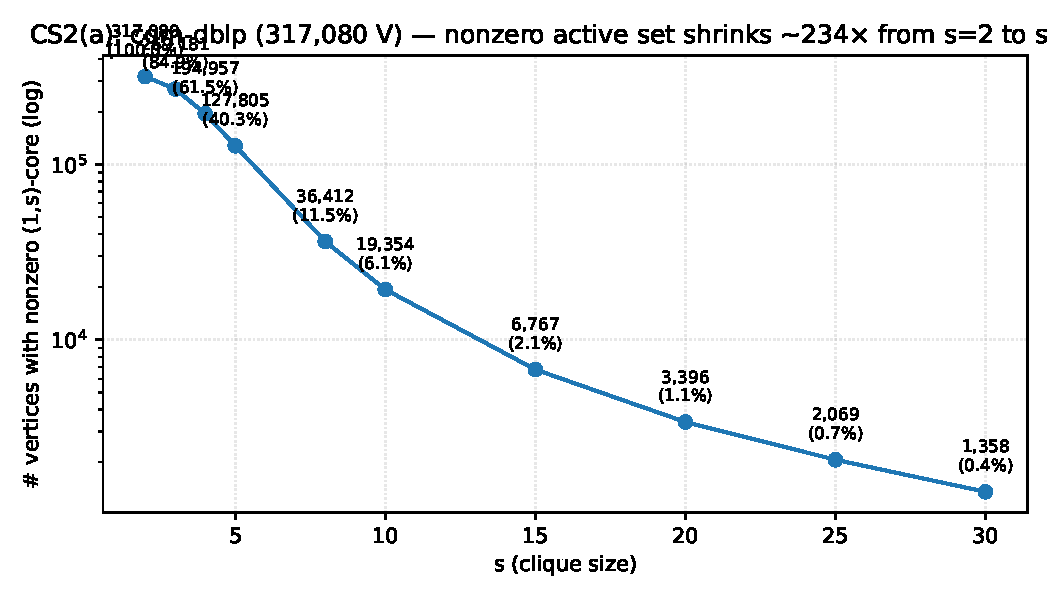
\includegraphics[width=0.95\linewidth]{figures/cs2_active_set.pdf}
\caption{Active-set size on \texttt{com-dblp} as \(s\) varies.
%
Observe that larger \(s\) sharply shrinks the vertices with nonzero \((1,s)\)-core value.}
\Description{Line plot showing the number of active vertices decreasing as clique size s increases.}
\label{fig:cs1}
\end{figure}

\stitle{Case study 2: \((1,s)\) improves the \(k\)-core ranking.}\label{sec:cs-quality}
On \texttt{com-dblp}, the first non-trivial clique support already improves the ground-truth ranking over \(k\)-core.
%
Table~\ref{tab:cs3} reports top-\(10{,}000\) quality.
%
Figure~\ref{fig:cs3} shows precision over \(K\).

\begin{table}[t]
\centering
\caption{Ground-truth quality of \((1,s)\)-cores versus \(k\)-core on \texttt{com-dblp}.}
\label{tab:cs3}
\small
\begin{tabular}{lrrrr}
\toprule
Method & top-\(K\) & Precision & rec50 & tri/v \\
\midrule
\(k\)-core      & \(10{,}000\) & \(0.504\) & \(94\)  & \(112.3\) \\
\((1,3)\)-core  & \(10{,}000\) & \(0.523\) & \(114\) & \(113.4\) \\
\((1,5)\)-core  & \(10{,}000\) & \(0.523\) & \(114\) & \(113.4\) \\
\((1,10)\)-core & \(10{,}000\) & \(0.523\) & \(114\) & \(113.4\) \\
\((1,15)\)-core & \(6{,}767\)  & \(\boldsymbol{0.548}\) & \(65\) & \(\boldsymbol{154}\) \\
\((1,30)\)-core & \(1{,}358\)  & \(0.507\) & \(4\) & \(\boldsymbol{523}\) \\
\bottomrule
\end{tabular}
\end{table}

\((1,3)\)-core raises precision from \(0.504\) to \(0.523\) and rec50 from \(94\) to \(114\).
%
For \(s\in\{3,5,10\}\), the top-\(10{,}000\) quality is identical in this table.
%
For larger \(s\), the active set drops below \(10{,}000\), so the comparison changes from ranking quality at fixed \(K\) to density of the surviving subgraph.
%
\((1,30)\)-core reaches \(523\) triangles per vertex on \(1{,}358\) vertices.

\begin{figure}[t]
\centering
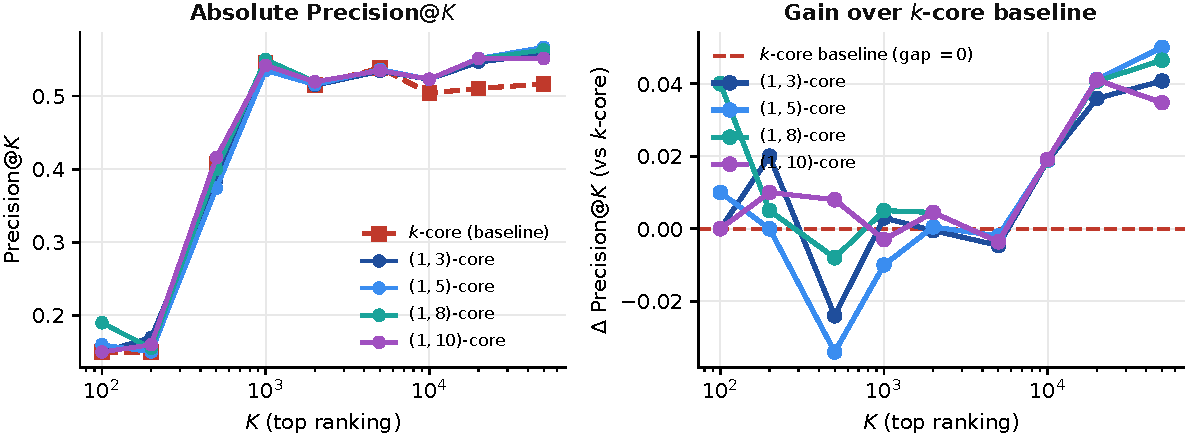
\includegraphics[width=\linewidth]{figures/cs3_precision.pdf}
\caption{Precision@\(K\) on \texttt{com-dblp}.
%
Observe that the \((1,s)\)-core rankings for \(s\in\{3,5,10,15\}\) stay above the \(k\)-core curve in the plotted range.}
\Description{Precision-at-K curves comparing k-core and several (1,s)-core rankings on DBLP.}
\label{fig:cs3}
\end{figure}

\stitle{Case study 3: higher \(r\) does not buy quality on DBLP.}\label{sec:cs-pareto}
The next question is whether edge-level or triangle-level nuclei improve the vertex ranking enough to justify their cost.
%
Table~\ref{tab:cs4} fixes \(s=10\) on \texttt{com-dblp}.
%
The \((1,10)\)-core and \((3,10)\)-core match on rec50 and triangle density, while \((1,10)\) is \(178\times\) faster in the reported run.

\begin{table}[t]
\centering
\caption{Cross-\(r\) comparison at \(s=10\) on \texttt{com-dblp}.}
\label{tab:cs4}
\small
\begin{tabular}{lrrrr}
\toprule
Method & Precision & rec50 & tri/v & Time (ms) \\
\midrule
\(k\)-core      & \(0.504\) & \(94\)  & \(112.3\) & \(2.3\) \\
\((1,10)\)-core & \(0.523\) & \(114\) & \(113.4\) & \(13.4\) \\
\((2,10)\)-core & \(0.529\) & \(113\) & \(71.8\)  & \(123.1\) \\
\((3,10)\)-core & \(0.524\) & \(114\) & \(113.4\) & \(2{,}379.6\) \\
\midrule
\textbf{(1) vs. (3)} & \(-0.001\) & \(0\) & \(0.0\) & \(-178\times\) \\
\bottomrule
\end{tabular}
\end{table}

The broader grid in Figure~\ref{fig:cs6} shows the same pattern on the reported DBLP settings.
%
The \(r=1\) frontier dominates the \(r\in\{2,3\}\) points in the plotted quality-runtime plane.
%
This does not prove higher \(r\) is never useful.
%
It shows that on this vertex-ranking task, increasing \(r\) mostly adds cost.

\begin{figure}[t]
\centering
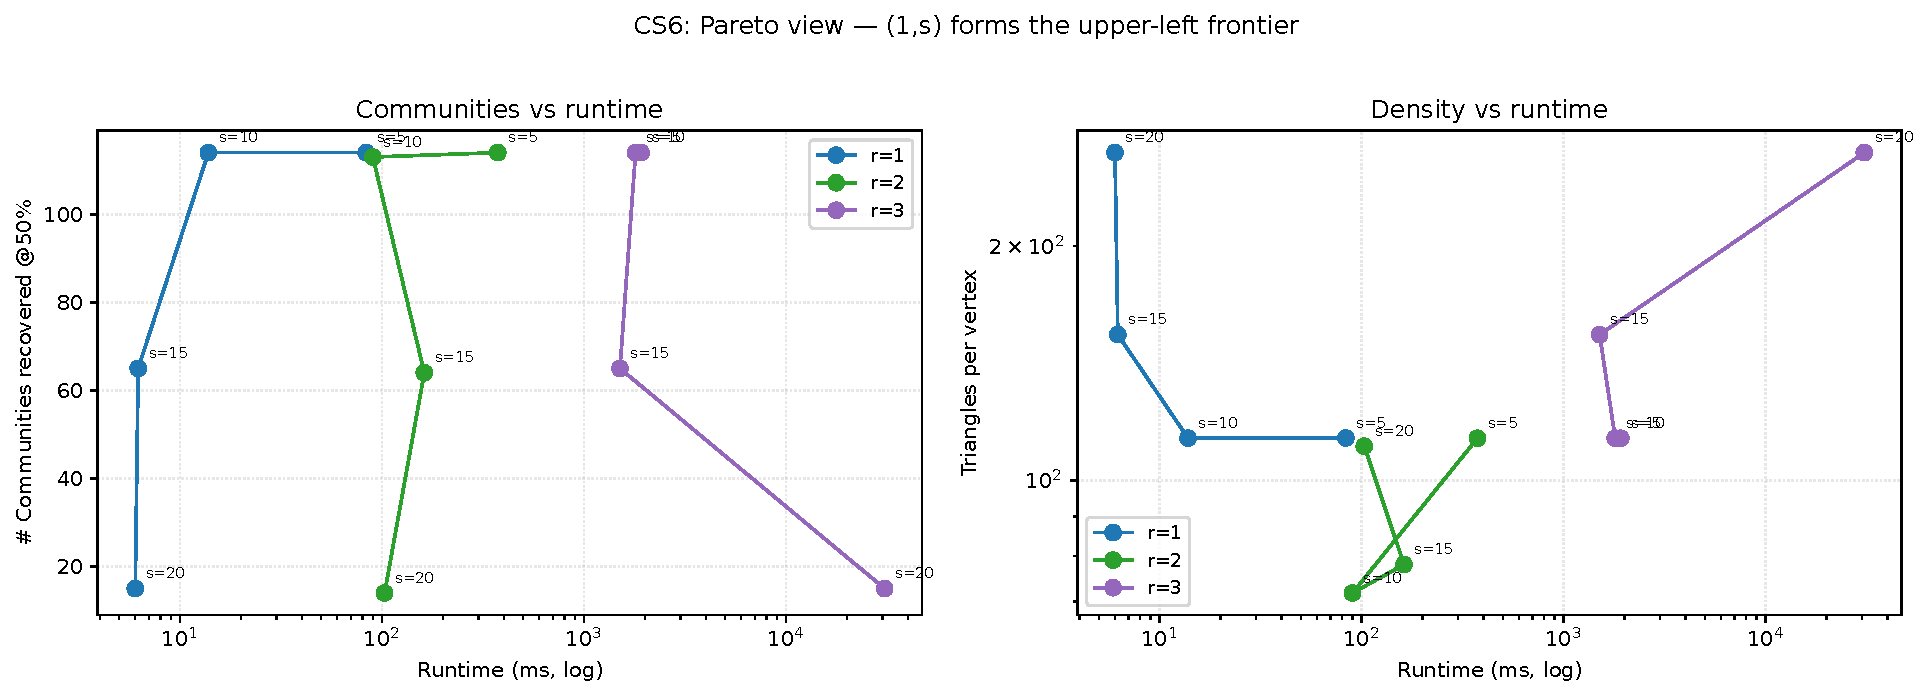
\includegraphics[width=\linewidth]{figures/cs6_pareto.pdf}
\caption{Quality-runtime Pareto plot on \texttt{com-dblp} for \(r\in\{1,2,3\}\) and \(s\in\{5,10,15,20\}\).
%
Observe that the \(r=1\) points lie on the favorable quality-runtime frontier in the DBLP settings.}
\Description{Scatter plot of quality versus runtime for several r and s settings on DBLP.}
\label{fig:cs6}
\end{figure}

\stitle{Case study 4: YouTube repeats the pattern.}\label{sec:cs-youtube}
The cross-\(r\) comparison is not limited to collaboration data.
%
Table~\ref{tab:cs7} reports the same comparison on \texttt{com-youtube}.
%
At \(s=10\), all three \(r\)-values match on rec50 and triangle density, while \(r=1\) is \(67.5\times\) faster than \(r=3\).

\begin{table}[t]
\centering
\caption{Cross-\(r\) comparison on \texttt{com-youtube}.}
\label{tab:cs7}
\small
\begin{tabular}{lrrrr}
\toprule
Method & rec50 & tri/v & Time (ms) & vs. \((1,s)\) \\
\midrule
\((1,5)\)  & \(283\) & \(173\) & \(274\)    & --- \\
\((2,5)\)  & \(286\) & \(161\) & \(2{,}580\) & \(9.4\times\) \\
\((3,5)\)  & \(288\) & \(159\) & \(13{,}112\) & \(47.9\times\) \\
\midrule
\((1,10)\) & \(49\) & \(293\) & \(31\)     & --- \\
\((2,10)\) & \(49\) & \(293\) & \(319\)    & \(10.3\times\) \\
\((3,10)\) & \(49\) & \(293\) & \(2{,}093\) & \(67.5\times\) \\
\midrule
\((1,15)\) & \(0^{\dagger}\) & \(173\) & \(9\)  & --- \\
\((2,15)\) & \(0^{\dagger}\) & \(173\) & \(55\) & \(6.2\times\) \\
\((3,15)\) & \(0^{\dagger}\) & \(173\) & \(87\) & \(9.8\times\) \\
\bottomrule
\end{tabular}
\\[2pt]\footnotesize \(^{\dagger}\)At \(s=15\), the active set has \(95\) vertices, below the smallest SNAP community size, so rec50 is zero for every method.
\end{table}

Figure~\ref{fig:cs7y} visualizes the same quality-runtime tradeoff.
%
The \(r=1\) points sit on the same quality contour as higher-\(r\) points but with lower runtime.

\begin{figure}[t]
\centering
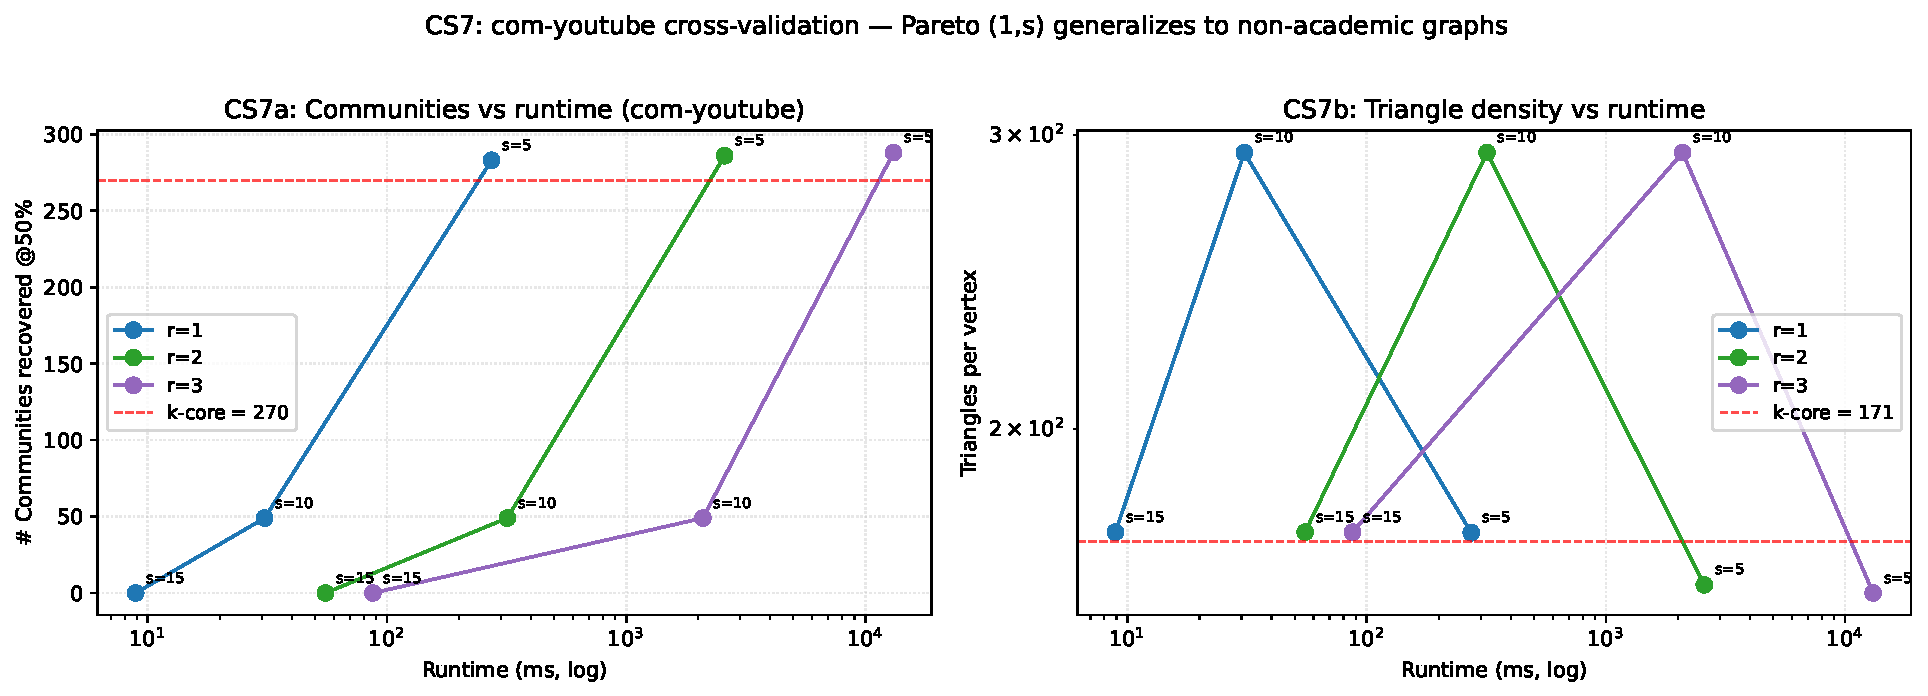
\includegraphics[width=0.95\linewidth]{figures/cs7_pareto.pdf}
\caption{Quality-runtime Pareto plot on \texttt{com-youtube} for \(r\in\{1,2,3\}\) and \(s\in\{5,10,15\}\).
%
Observe that \(r=1\) reaches the same quality contours as higher-\(r\) settings with lower runtime.}
\Description{Scatter plot of quality versus runtime for several r and s settings on YouTube.}
\label{fig:cs7y}
\end{figure}

\stitle{Case study 5: \(s\) changes local resolution.}\label{sec:cs-viz}
The previous studies use global rankings.
%
The ego-network visualization asks whether \(s\) also changes local interpretability.
%
Figure~\ref{fig:cs9} shows the two-hop ego-network of \texttt{com-dblp} vertex \(52213\) under \(s\in\{3,5,10\}\).
%
Table~\ref{tab:cs9} reports the component statistics.

\begin{table}[t]
\centering
\caption{Ego-network of \texttt{com-dblp} anchor \(52213\) under three \(s\) values.}
\label{tab:cs9}
\small
\begin{tabular}{r r r r r r}
\toprule
\(s\) & \(|V|\) & CCs & largest CC & intra-frac & avg cond \\
\midrule
\(3\)  & \(462\) & \(1\)  & \(462\) & \(0.992\) & \(0.004\) \\
\(5\)  & \(335\) & \(5\)  & \(329\) & \(0.796\) & \(0.121\) \\
\(10\) & \(66\)  & \(26\) & \(32\)  & \(0.340\) & \(0.636\) \\
\bottomrule
\end{tabular}
\end{table}

At \(s=3\), the ego-network remains one large component.
%
At \(s=10\), it becomes \(26\) smaller components.
%
This behavior makes \(s\) a local resolution knob.

\begin{figure}[t]
\centering
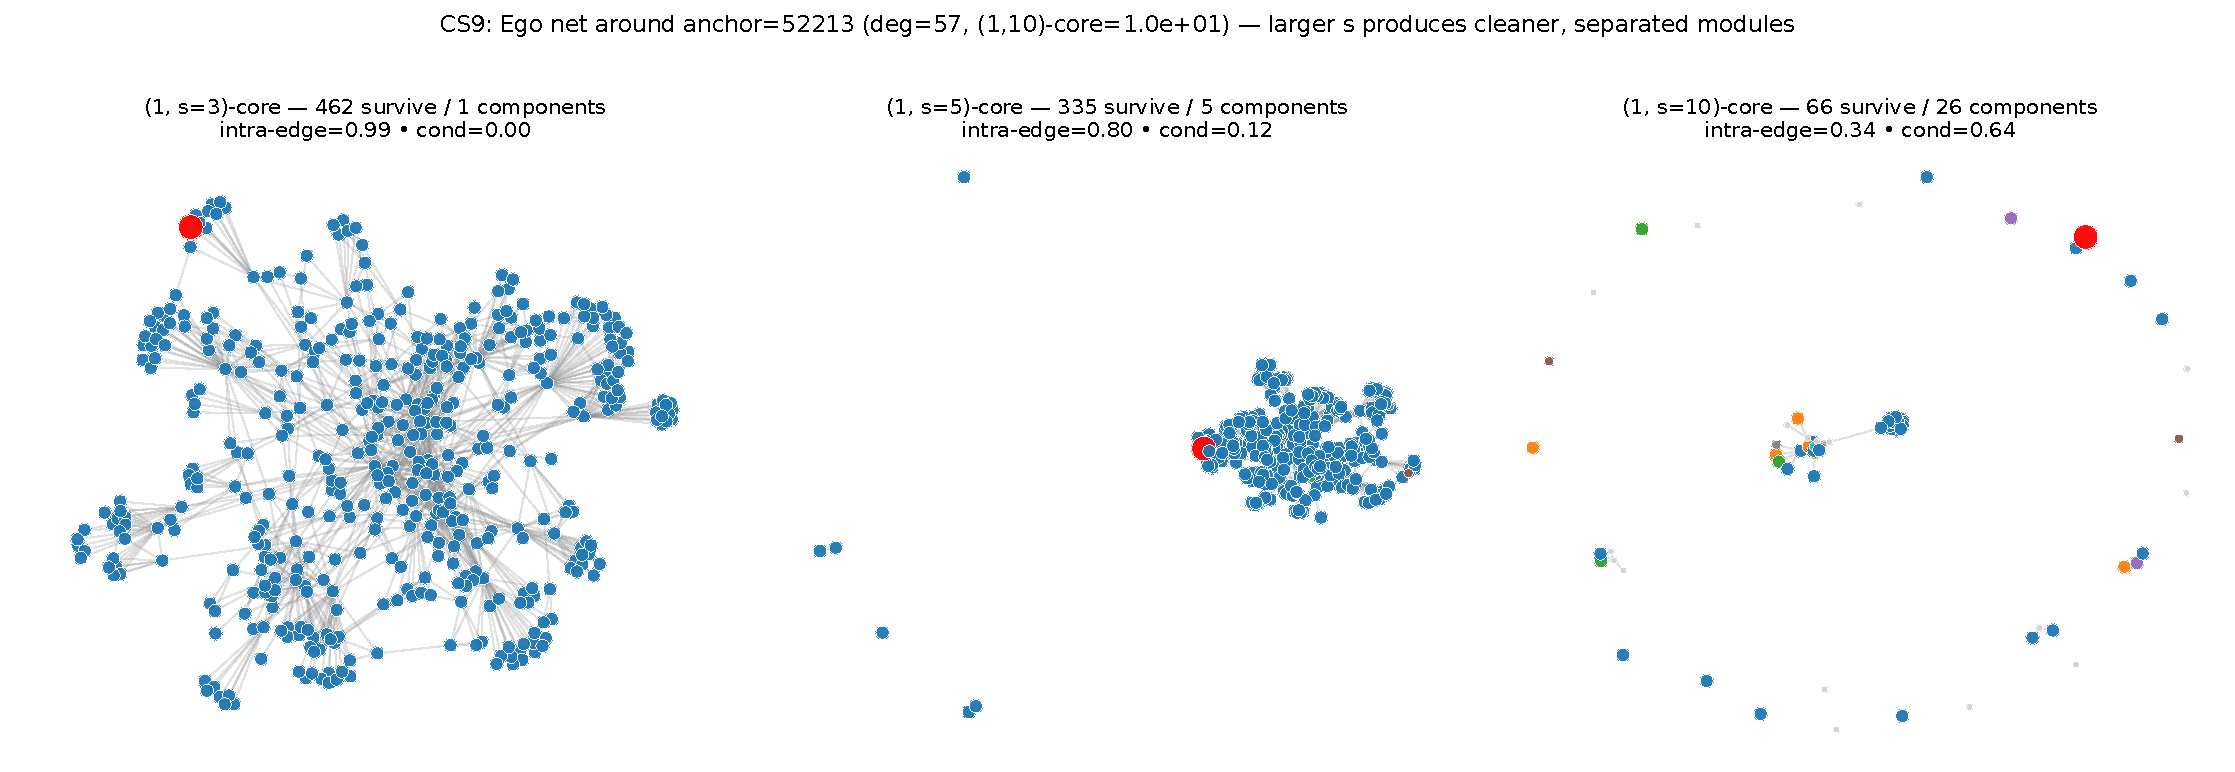
\includegraphics[width=\linewidth]{figures/cs9_egonet.pdf}
\caption{Two-hop ego-network of a \texttt{com-dblp} anchor under \((1,s)\)-decomposition.
%
Vertices are colored by connected component among surviving vertices.
%
Observe that increasing \(s\) splits one large local structure into smaller components.}
\Description{Three ego-network visualizations showing components becoming smaller and more numerous as s increases.}
\label{fig:cs9}
\end{figure}

\stitle{Case study 6: hierarchy profiles differ by domain.}\label{sec:cs-hier}
\buildHier{} turns the core values into an edge-connected super-level join tree.
%
This makes it possible to compare how quickly the core-value hierarchy collapses across domains.
%
Table~\ref{tab:cs10cross} reports the three hierarchy statistics used here.
%
Figures~\ref{fig:cs10} and~\ref{fig:cs10p} visualize the resulting trees and persistence diagrams.

\begin{table}[t]
\centering
\caption{Edge-connected core-value hierarchy summary.
%
The table reports branches, internal absorption events, and maximum tree depth.}
\label{tab:cs10cross}
\tiny
\setlength{\tabcolsep}{2pt}
\begin{tabular}{@{}l rrr rrr rrr rrr@{}}
\toprule
& \multicolumn{3}{c}{\(s=3\)} & \multicolumn{3}{c}{\(s=5\)} & \multicolumn{3}{c}{\(s=10\)} & \multicolumn{3}{c}{\(s=15\)} \\
\cmidrule(lr){2-4}\cmidrule(lr){5-7}\cmidrule(lr){8-10}\cmidrule(lr){11-13}
graph & br. & int. & d & br. & int. & d & br. & int. & d & br. & int. & d \\
\midrule
\texttt{com-dblp}     & \(9{,}968\) & \(1{,}175\) & \(8\) & \(5{,}794\) & \(583\) & \(7\) & \(664\) & \(8\) & \(1\) & \(222\) & \(2\) & \(1\) \\
\texttt{com-youtube}  & \(3{,}568\) & \(61\) & \(2\) & \(280\) & \(1\) & \(1\) & \(14\) & \(0\) & \(0\) & -- & -- & -- \\
\texttt{web-Stanford} & \(8{,}731\) & \(1{,}776\) & \(7\) & \(6{,}473\) & \(1{,}032\) & \(8\) & \(1{,}946\) & \(277\) & \(3\) & \(1{,}573\) & \(220\) & \(2\) \\
\bottomrule
\end{tabular}
\end{table}

\texttt{com-youtube} collapses quickly.
%
\texttt{com-dblp} keeps nontrivial structure until roughly \(s=10\).
%
\texttt{web-Stanford} retains many branches even at \(s=15\).
%
The hierarchy is therefore not only an output format.
%
It gives a domain-level fingerprint of core-value nesting.

\begin{figure}[t]
\centering
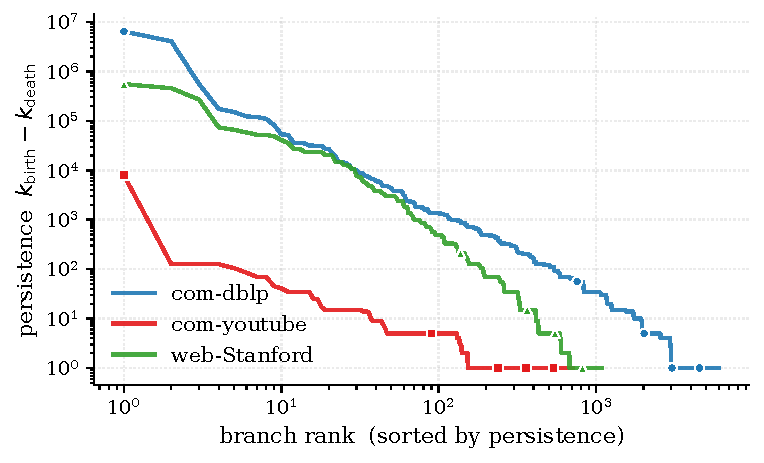
\includegraphics[width=\linewidth]{figures/cs10_hierarchy.pdf}
\caption{Edge-connected core-value join tree at \(s=5\) across three domains.
%
Observe that the hierarchy shapes differ across collaboration, social, and web graphs.}
\Description{Three hierarchy-tree visualizations comparing DBLP, YouTube, and web-Stanford at s equals 5.}
\label{fig:cs10}
\end{figure}

\begin{figure}[t]
\centering
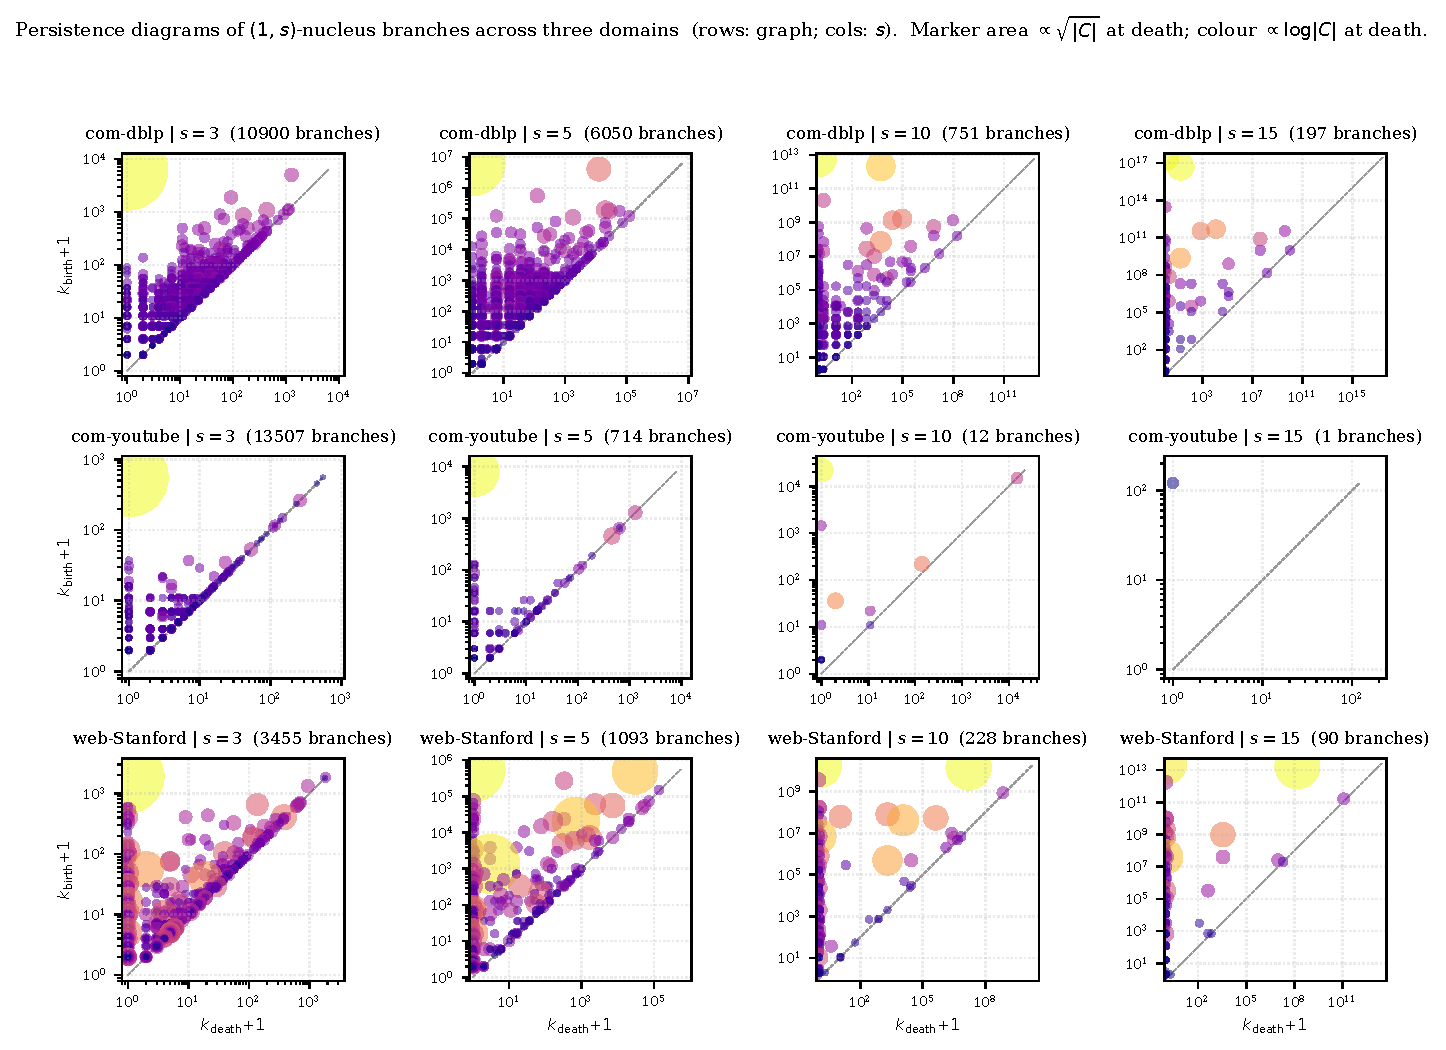
\includegraphics[width=\linewidth]{figures/cs10_persistence.pdf}
\caption{Persistence diagrams across three domains and four \(s\) values.
%
Observe that branch persistence changes with both domain and clique size.}
\Description{Grid of persistence diagrams for three domains and four clique-size settings.}
\label{fig:cs10p}
\end{figure}

\stitle{Case study 7: clique-coherent hierarchy.}\label{sec:cs-clique}
The hierarchy above uses edge connectivity among surviving vertices.
%
A more clique-faithful variant connects two vertices at level \(k\) only when they co-occur in an \(s\)-clique whose vertices all have core value at least \(k\).
%
This variant uses the same \cpi{} representation as the decomposition, because the \(s\)-cliques are the connectivity witnesses.
%
Figure~\ref{fig:cs10b} shows the difference.
%
% TODO: verify the clique-coherent counts before restoring a numeric comparison.

\begin{figure}[t]
\centering
\includegraphics[width=\linewidth]{figures/cs10b_compare.pdf}
\caption{Edge-based versus clique-coherent persistence diagrams on \texttt{com-dblp} at \(s=3\).
%
Observe that changing the connectivity witness changes the branch profile.}
\Description{Two persistence diagrams comparing edge-based and clique-coherent hierarchy definitions.}
\label{fig:cs10b}
\end{figure}

\stitle{Takeaway.}\label{sec:cs-summary}
These studies support the paper's focus on \((1,s)\).
%
The parameter \(s\) changes granularity.
%
On the reported DBLP and YouTube ground-truth tasks, \(r=1\) matches higher-\(r\) quality metrics while running much faster.
%
The hierarchy and ego-network studies show that the same vertex-centric decomposition also gives interpretable structure beyond a global ranking.
%
The evidence is not a universal claim about all graph mining tasks.
%
It is a practical justification for optimizing the exact \(r=1\) case.
